% This file was created by tikzplotlib v0.9.2.
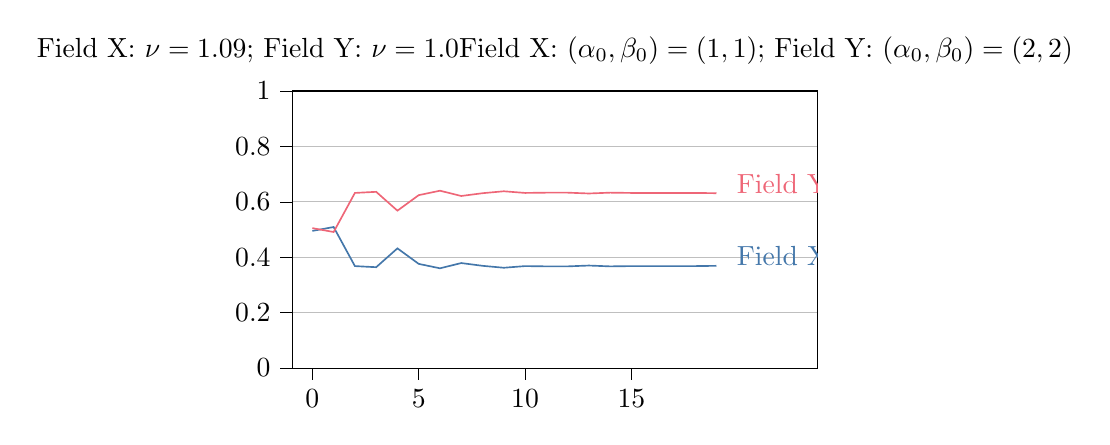
\begin{tikzpicture}

\definecolor{color0}{rgb}{0.266666666666667,0.466666666666667,0.666666666666667}
\definecolor{color1}{rgb}{0.933333333333333,0.4,0.466666666666667}

\begin{axis}[
height=5.101085673964669cm,
tick align=outside,
tick pos=left,
title={Field X: \(\displaystyle \nu=1.09\); Field Y: \(\displaystyle \nu=1.0\) \\ Field X: \(\displaystyle (\alpha_0, \beta_0)=(1, 1)\); Field Y: \(\displaystyle (\alpha_0, \beta_0)=(2, 2)\)},
width=8.25373cm,
x grid style={white!69.0196078431373!black},
xmin=-0.95, xmax=23.75,
xtick style={color=black},
xtick={0,5,10,15},
xticklabels={\(\displaystyle 0\),\(\displaystyle 5\),\(\displaystyle 10\),\(\displaystyle 15\)},
ymajorgrids,
ymin=0, ymax=1,
ytick style={color=black},
ytick={0,0.2,0.4,0.6,0.8,1},
yticklabels={\(\displaystyle 0\),\(\displaystyle 0.2\),\(\displaystyle 0.4\),\(\displaystyle 0.6\),\(\displaystyle 0.8\),\(\displaystyle 1\)}
]
\addplot [semithick, color0]
table {%
0 0.495
1 0.509
2 0.368
3 0.364
4 0.432
5 0.376
6 0.36
7 0.379
8 0.369
9 0.362
10 0.368
11 0.367
12 0.367
13 0.37
14 0.367
15 0.368
16 0.368
17 0.368
18 0.368
19 0.369
};
\addplot [semithick, color1]
table {%
0 0.505
1 0.491
2 0.632
3 0.636
4 0.568
5 0.624
6 0.64
7 0.621
8 0.631
9 0.638
10 0.632
11 0.633
12 0.633
13 0.63
14 0.633
15 0.632
16 0.632
17 0.632
18 0.632
19 0.631
};
\draw (axis cs:19.5,0.369) node[
  anchor=base west,
  text=color0,
  rotate=0.0
]{Field X};
\draw (axis cs:19.5,0.631) node[
  anchor=base west,
  text=color1,
  rotate=0.0
]{Field Y};
\end{axis}

\end{tikzpicture}
